\documentclass[a4page]{article}
\usepackage[14pt]{extsizes} % для того чтобы задать нестандартный 14-ый размер шрифта
\usepackage[utf8]{inputenc}
\usepackage[T1, T2A]{fontenc}
\usepackage[utf8]{inputenc}
\usepackage[russian]{babel} % поддержка русского языка
\usepackage{amsmath}  %  математические символы
\usepackage[left=25mm, top=20mm, right=15mm, bottom=30mm, footskip=15mm]{geometry} % настройки полей документа
\usepackage{indentfirst} % по умалчанию убирается отступ у первого абзаца в секции, это отменяет это.
\usepackage{paralist} % добавить компактные списки (compactitem, compactenum, compactdesc)

\usepackage{fancyvrb}
\usepackage{fancyref}
\usepackage{framed}
\usepackage{url}
\usepackage{csquotes}
\usepackage{listings}

\usepackage{graphicx}
\graphicspath{ {./Images/} }

\usepackage{float}
\floatstyle{ruled}

\usepackage[
	backend=biber,
	sorting=nyt,
	bibstyle=gost-numeric,
	citestyle=gost-numeric
]{biblatex}

\usepackage[
	bookmarks=true, colorlinks=true, unicode=true,
	urlcolor=black,linkcolor=black, anchorcolor=black,
	citecolor=black, menucolor=black, filecolor=black,
]{hyperref}

\addbibresource{sources.bib}

\renewcommand{\baselinestretch}{1.25}

\begin{document}

\begin{titlepage}
	\begin{center}
		\hfill \break
		\textbf{
			\large{РОССИЙСКИЙ УНИВЕРСИТЕТ ДРУЖБЫ НАРОДОВ}\\
			\normalsize{Факультет физико-математических и естественных наук}\\
			\normalsize{Кафедра прикладной информатики и теории вероятностей}\\
		}
		\vspace*{\fill}
		\Large{\textbf{Архитектура REST взаимодействия компонентов распределённого приложения в сети.\\Обозначение объектов JavaScript (JSON).}}
		\\
		\underline{\textit{\normalsize{Дисциплина: Вычислительные системы, сети и телекоммуникации}}}
		\vspace*{\fill}

	\end{center}

	\begin{flushright}
		Студент: \underline{Матюхин Григорий}\\ \vspace{0.5cm}
		Группа: \underline{НПИбд-01-21}
	\end{flushright}

	\begin{center} \textbf{МОСКВА} \\ 2023 г. \end{center}
	\thispagestyle{empty}

\end{titlepage}

\newpage

\tableofcontents

\newpage
\section{Введение}

\newpage
\section{REST}
REST (от англ. Representational State Transfer ---
<<передача репрезентативного состояния>> или <<передача "самоописываемого" состояния>>) ---
архитектурный стиль взаимодействия компонентов распределённого приложения в сети \cite{REST}.
Другими словами, REST --- это набор правил того,
как программисту организовать написание кода серверного приложения,
чтобы все системы легко обменивались данными и приложение можно было масштабировать.
REST представляет собой согласованный набор ограничений,
учитываемых при проектировании распределённой гипермедиа-системы.

Для веб-служб, построенных с учётом REST (то есть не нарушающих накладываемых им ограничений),
применяют термин <<RESTful>>.

\subsection{Свойства архитектуры REST}
Архитектурный стиль REST разработан для сетевых приложений,
в частности для клиент-серверных приложений.
Но более того, он предназначен для использования в масштабах Интернета,
поэтому связь между пользовательским агентом (клиентом) и
исходным сервером должна быть как можно более свободной, чтобы способствовать широкомасштабному внедрению.

Сильное разделение клиента и сервера вместе с текстовой передачей информации
с использованием единого протокола адресации послужило основой для удовлетворения требований Интернета:
надежность (анархическая масштабируемость), независимое развертывание компонентов,
крупнозернистая передача данных и низкий входной барьер для читателей контента,
авторов контента и разработчиков.

Ограничения архитектурного стиля REST влияют на следующие архитектурные свойства:

\begin{itemize}
	\item производительность при взаимодействии компонентов,
	      которая может быть доминирующим фактором воспринимаемой пользователем производительности и эффективности сети;
	\item масштабируемость, позволяющая поддерживать большое количество компонентов
	      и взаимодействие между компонентами;
	\item простота единого интерфейса;
	\item модифицируемость компонентов для удовлетворения меняющихся потребностей
	      (даже во время работы приложения);
	\item видимость связи между компонентами сервисными агентами;
	\item переносимость компонентов за счет перемещения программного кода вместе с данными;
	\item надежность в устойчивости к сбоям на системном уровне при наличии сбоев в компонентах,
	      соединителях или данных.
\end{itemize}

\subsection{Требования к архитектуре REST}
Существует шесть обязательных ограничений для построения распределённых REST-приложений по Филдингу.

Выполнение этих ограничений обязательно для REST-систем.
Накладываемые ограничения определяют работу сервера в том,
как он может обрабатывать и отвечать на запросы клиентов.
Действуя в рамках этих ограничений,
система приобретает такие желательные свойства как производительность,
масштабируемость, простота, способность к изменениям, переносимость, отслеживаемость и надёжность.

Если сервис-приложение нарушает любое из этих ограничительных условий,
данную систему нельзя считать REST-системой.

Обязательными условиями-ограничениями являются:

\subsubsection{Модель клиент-сервер}
Шаблон проектирования клиент-сервер реализует принцип разделения задач:
отделение задач пользовательского интерфейса от задач хранения данных.
Таким образом, повышается переносимость пользовательского интерфейса.
В случае с Интернетом для большинства платформ было разработано множество веб-браузеров
без необходимости знания каких-либо серверных реализаций.
Разделение также упрощает серверные компоненты, улучшая масштабируемость,
но, что более важно, оно позволяет компонентам развиваться независимо (анархическая масштабируемость),
что необходимо в среде интернет-масштаба, включающей несколько организационных доменов.

\subsubsection{Отсутствие состояния}
Протокол взаимодействия между клиентом и сервером требует соблюдения следующего условия:
в период между запросами клиента никакая информация о состоянии клиента на сервере не хранится
(Stateless protocol или «протокол без сохранения состояния»).
Все запросы от клиента должны быть составлены так,
чтобы сервер получил всю необходимую информацию для выполнения запроса.
Состояние сессии при этом сохраняется на стороне клиента.
Информация о состоянии сессии может быть передана сервером какому-либо другому сервису
(например, в службу базы данных) для поддержания устойчивого состояния,
например, на период установления аутентификации.
Клиент инициирует отправку запросов, когда он готов (возникает необходимость) перейти в новое состояние.

\subsubsection{Кэширование}
Как и во всемирной паутине, клиенты и посредники могут кэшировать ответы.
Ответы должны явно или неявно определять себя как кэшируемые или некэшируемые,
чтобы клиенты не предоставляли устаревшие или неподходящие данные в ответ на дальнейшие запросы.
Хорошо управляемое кэширование частично или полностью устраняет некоторые взаимодействия
между клиентом и сервером, дополнительно повышая масштабируемость и производительность.
Кэширование может выполняться на клиентской машине в памяти или в хранилище кеша браузера.
Кроме того, кэш может храниться в сети доставки контента (CDN).

\subsubsection{Единообразие интерфейса}
Ограничение единого интерфейса имеет основополагающее значение для проектирования любой системы RESTful.
Он упрощает и разделяет архитектуру, что позволяет каждой части развиваться независимо.
Четыре ограничения для этого универсального интерфейса:

\begin{itemize}
	\item Идентификация ресурсов в запросах.
	      Отдельные ресурсы идентифицируются в запросах, например, с помощью URI в веб-службах RESTful.
	      Сами ресурсы концептуально отделены от представлений, возвращаемых клиенту.
	      Например, сервер может отправлять данные из своей базы данных в формате HTML,
	      XML или JSON, ни один из которых не является внутренним представлением сервера.
	\item Манипулирование ресурсами с помощью представлений.
	      Когда клиент содержит представление ресурса, включая любые прикрепленные метаданные,
	      у него достаточно информации для изменения или удаления состояния ресурса.
	\item Самоописательные сообщения.
	      Каждое сообщение содержит достаточно информации, чтобы описать, как его обрабатывать.
	      Например, какой синтаксический анализатор вызывать, можно определить по типу носителя.
	\item Гипермедиа как механизм состояния приложения (HATEOAS).
	      Получив доступ к начальному URI для приложения REST --- аналогично тому,
	      как пользователь Web-человека получает доступ к домашней странице веб-сайта, ---
	      клиент REST должен иметь возможность динамически использовать предоставленные сервером ссылки
	      для обнаружить все доступные ресурсы, в которых он нуждается.
	      Когда доступ продолжается, сервер отвечает текстом, который включает гиперссылки на другие ресурсы,
	      доступные в данный момент. Клиенту не нужно жестко запрограммировать информацию о структуре сервера
	      (подробнее см. секцию \ref{hateoas}).
\end{itemize}

\subsubsection{Слои}
Клиент обычно не может сказать, подключен ли он напрямую к конечному серверу или к посреднику по пути.
Если между клиентом и сервером размещен прокси-сервер или балансировщик нагрузки,
это не повлияет на их связь, и не потребуется обновлять код клиента или сервера.
Промежуточные серверы могут улучшить масштабируемость системы,
обеспечивая балансировку нагрузки и общие кэши.
Кроме того, безопасность можно добавить как уровень поверх веб-сервисов,
отделив бизнес-логику от логики безопасности.
Добавление безопасности в качестве отдельного уровня обеспечивает соблюдение политик безопасности.
Наконец, промежуточные серверы могут вызывать несколько других серверов, чтобы сгенерировать ответ клиенту.

\subsubsection{Код по требованию}
REST может позволить расширить функциональность клиента за счёт загрузки кода с сервера
в виде апплетов или скриптов. Филдинг утверждает,
что дополнительное ограничение позволяет проектировать архитектуру,
поддерживающую желаемую функциональность в общем случае, но, возможно, за исключением некоторых контекстов.

\subsection{HATEOAS}\label{hateoas}
Гипермедиа как механизм состояния приложения (HATEOAS) --- это ограничение архитектуры приложений REST,
которое отличает ее от других архитектур сетевых приложений.
С HATEOAS клиент взаимодействует с сетевым приложением,
чьи серверы приложений динамически предоставляют информацию через гипермедиа.
Клиенту REST практически не нужны предварительные знания о том,
как взаимодействовать с приложением или сервером, помимо общего понимания гипермедиа.
Напротив, клиенты и серверы в архитектуре Common Object Request Broker (CORBA)
взаимодействуют через фиксированный интерфейс,
совместно используемый через документацию или язык описания интерфейса (IDL).
Ограничения, налагаемые HATEOAS, разделяют клиент и сервер.
Это позволяет функциональности сервера развиваться независимо.

\subsubsection{Пример}
Пользовательский агент отправляет HTTP-запрос к REST API через URL-адрес точки входа.
Все последующие запросы, которые может сделать пользовательский агент,
обнаруживаются внутри ответа на каждый запрос.
Типы мультимедиа, используемые для этих представлений, и отношения ссылок, которые они могут содержать,
являются частью API. Клиент переходит через состояния приложения,
выбирая из ссылок в представлении или манипулируя представлением другими способами,
предоставляемыми его типом носителя.
Таким образом, RESTful-взаимодействие управляется гипермедиа,
а не внешней информацией \cite{REST-hyper}.

Например, этот запрос GET извлекает ресурс учетной записи, запрашивая детали в представлении JSON:
\begin{lstlisting}
GET /accounts/12345 HTTP/1.1
Host: bank.example.com
\end{lstlisting}

Ответ:

\begin{lstlisting}
HTTP/1.1 200 OK

{
    "account": {
        "account_number": 12345,
        "balance": {
            "currency": "usd",
            "value": 100.00
        },
        "links": {
            "deposits": "/accounts/12345/deposits",
            "withdrawals": "/accounts/12345/withdrawals",
            "transfers": "/accounts/12345/transfers",
            "close-requests": "/accounts/12345/close-requests"
        }
    }
}
\end{lstlisting}

Ответ содержит следующие возможные последующие ссылки:
POST депозит, снятие средств, перевод или запрос на закрытие (закрыть учетную запись).

Например, позже, после перерасхода учетной записи,
будет другой набор доступных ссылок, потому что учетная запись перерасходована.

\begin{lstlisting}
HTTP/1.1 200 OK

{
    "account": {
        "account_number": 12345,
        "balance": {
            "currency": "usd",
            "value": -25.00
        },
        "links": {
            "deposits": "/accounts/12345/deposits"
        }
    }
}
\end{lstlisting}

Сейчас доступна только одна ссылка: внести больше денег (путем POSTing на депозиты).
В текущем состоянии другие ссылки недоступны.
Отсюда и термин «механизм состояния приложения». Возможные действия зависят от состояния ресурса.

Клиенту не нужно понимать каждый тип мультимедиа и механизм связи, предлагаемый сервером.
Способность понимать новые типы мультимедиа может быть получена во время выполнения
с помощью <<кода по запросу>>, предоставляемого клиенту сервером.

\subsection{Преимущества}
Рой Филдинг указывал, что приложения, не соответствующие приведённым условиям,
не могут называться REST-приложениями. Если же все условия соблюдены, то, по его мнению,
приложение получит следующие преимущества:

\begin{itemize}
	\item Надёжность (за счёт отсутствия необходимости сохранять информацию о состоянии клиента,
	      которая может быть утеряна);
	\item Производительность (за счёт использования кэша);
	\item Масштабируемость;
	\item Прозрачность системы взаимодействия (особенно необходимая для приложений обслуживания сети);
	\item Простота интерфейсов;
	\item Портативность компонентов;
	\item Лёгкость внесения изменений;
	\item Способность эволюционировать, приспосабливаясь к новым требованиям (на примере Всемирной паутины).
\end{itemize}

\subsection{Недостатки}

\newpage
\section{JSON}
JSON (англ. JavaScript Object Notation) ---
текстовый формат обмена данными, основанный на JavaScript \cite{rfc8259}\cite{ISO21778}.
Как и многие другие текстовые форматы, JSON легко читается людьми.
Формат JSON был разработан Дугласом Крокфордом.

Несмотря на происхождение от JavaScript
(точнее, от подмножества языка стандарта ECMA-262 1999 \cite{ecma:262} года),
формат считается независимым от языка и может использоваться практически с любым языком программирования.
Для многих языков существует готовый код для создания и обработки данных в формате JSON.

\subsection{Синтаксис}
JSON построен на двух структурах:

\begin{itemize}
	\item Коллекция пар имя/значение.
	      В различных языках это реализуется как объект, запись, структура, словарь, хеш-таблица,
	      список с ключами или ассоциативный массив.
	\item Упорядоченный список значений.
	      В большинстве языков это реализовано в виде массива, вектора, списка или последовательности.
\end{itemize}

Это универсальные структуры данных. Практически все современные языки программирования поддерживают их
в той или иной форме. Имеет смысл, чтобы формат данных, взаимозаменяемый с языками программирования,
также основывался на этих структурах.

В JSON они принимают следующие виды (см. \hyperref[appendix]{приложение А}):
\begin{itemize}
	\item \textit{Объект} представляет собой неупорядоченный набор пар имя/значение.
	      Объект начинается с $\{_{\textup{левой скобки}}$ и заканчивается $\}_{\textup{правой скобкой}}$.
	      За каждым именем следует $:_\textup{двоеточие}$, а пары имя/значение разделяются $,_\textup{запятой}$.
	\item \textit{Массив} --- это упорядоченный набор значений.
	      Массив начинается с $[_{\textup{левой скобки}}$ и заканчивается $]_{\textup{правой скобкой}}$.
	      Значения разделяются $,_\textup{запятой}$.
	\item \textit{Значение} может быть \textit{строкой} в двойных кавычках,
	      или \textit{числом}, или \texttt{true}, или \texttt{false}, или \texttt{null}, или \textit{объектом},
	      или \textit{массивом}. Эти структуры могут быть вложенными.
	\item \textit{Строка} --- это последовательность из нуля или более символов Юникода,
	      заключенная в двойные кавычки и использующая символы обратной косой черты.
	      Один символ представлен в виде строки из одного элемента.
	\item \textit{Число} очень похоже на число C или Java, за исключением того,
	      что восьмеричный и шестнадцатеричный форматы не используются.
	\item \textit{Пробелы} могут быть вставлены между любой парой токенов.
\end{itemize}

За исключением нескольких деталей кодировки, это полностью описывает язык.

\subsection{YAML}

\subsection{Расширения в RESTful архитектуре}

\subsubsection{HAL}

\subsubsection{JSON-LD}

\newpage
\section{Заключение}

\newpage
\addcontentsline{toc}{section}{Приложение А. Синтаксические диаграммы JSON}
\section*{Приложение А. Синтаксические диаграммы JSON} \label{appendix}
\begin{enumerate}
	\item Объект \\
	      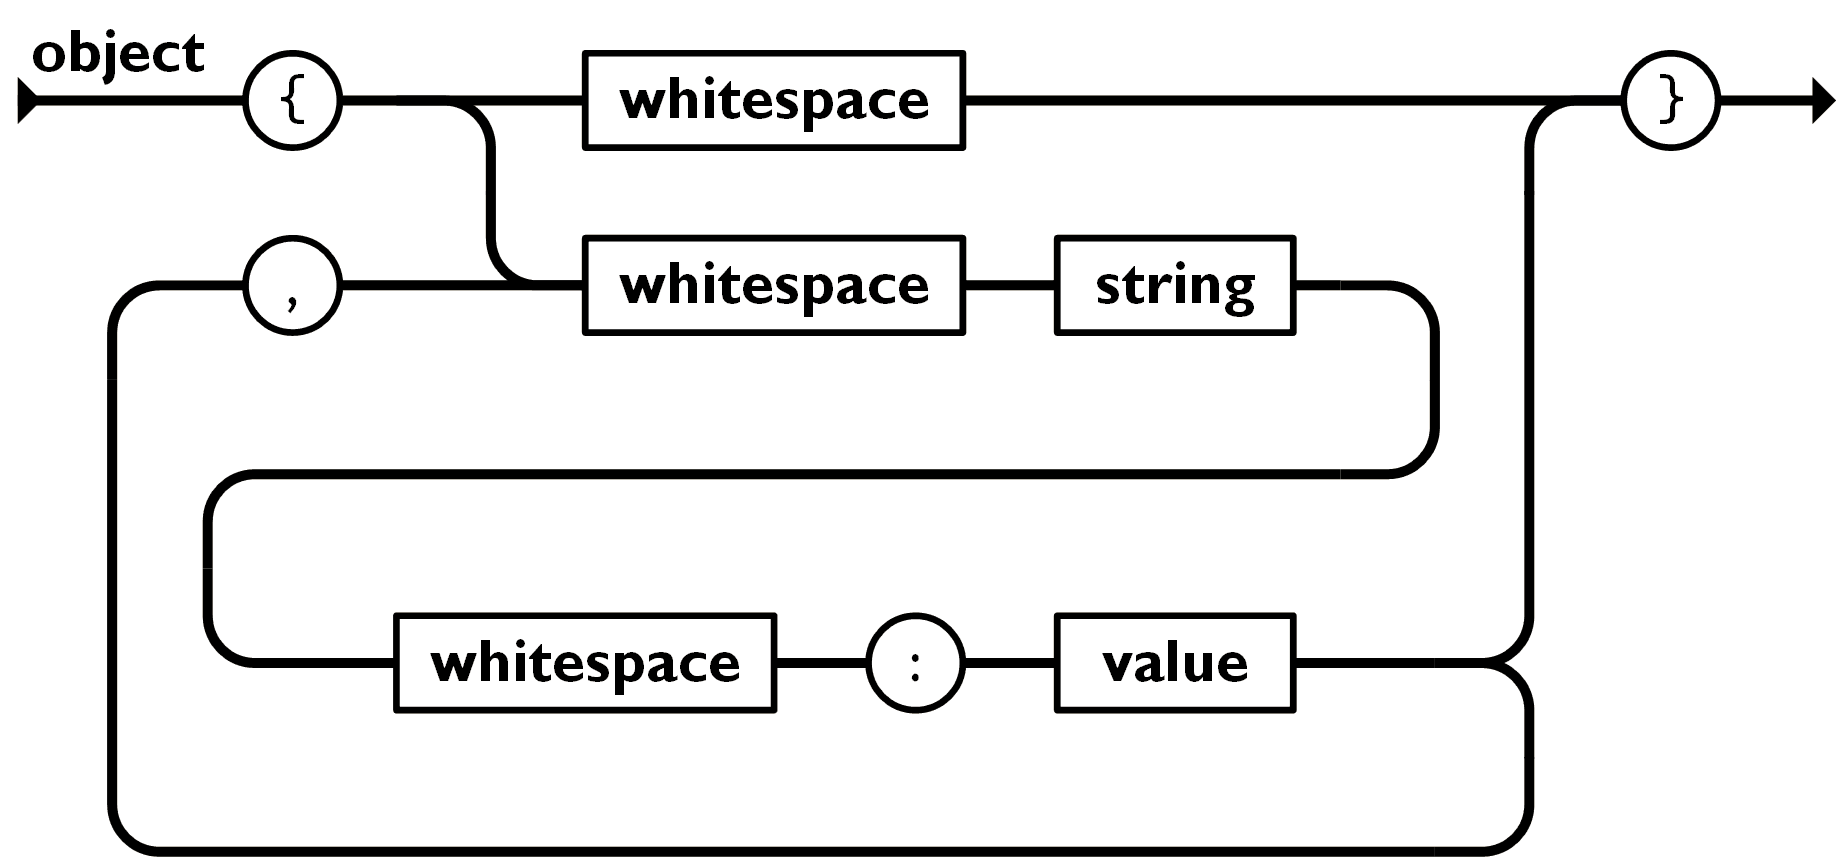
\includegraphics[scale=0.6]{object.png}
	\item Массив \\
	      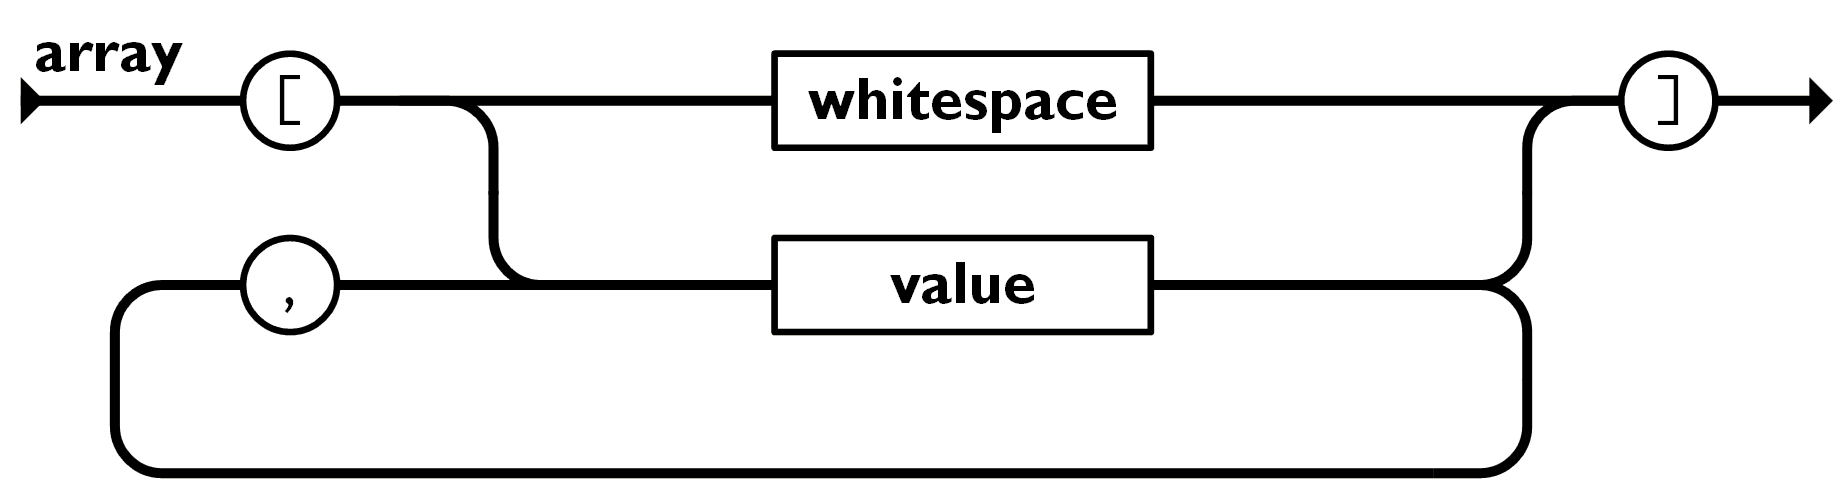
\includegraphics[scale=0.6]{array.png}
	\item Значение \\
	      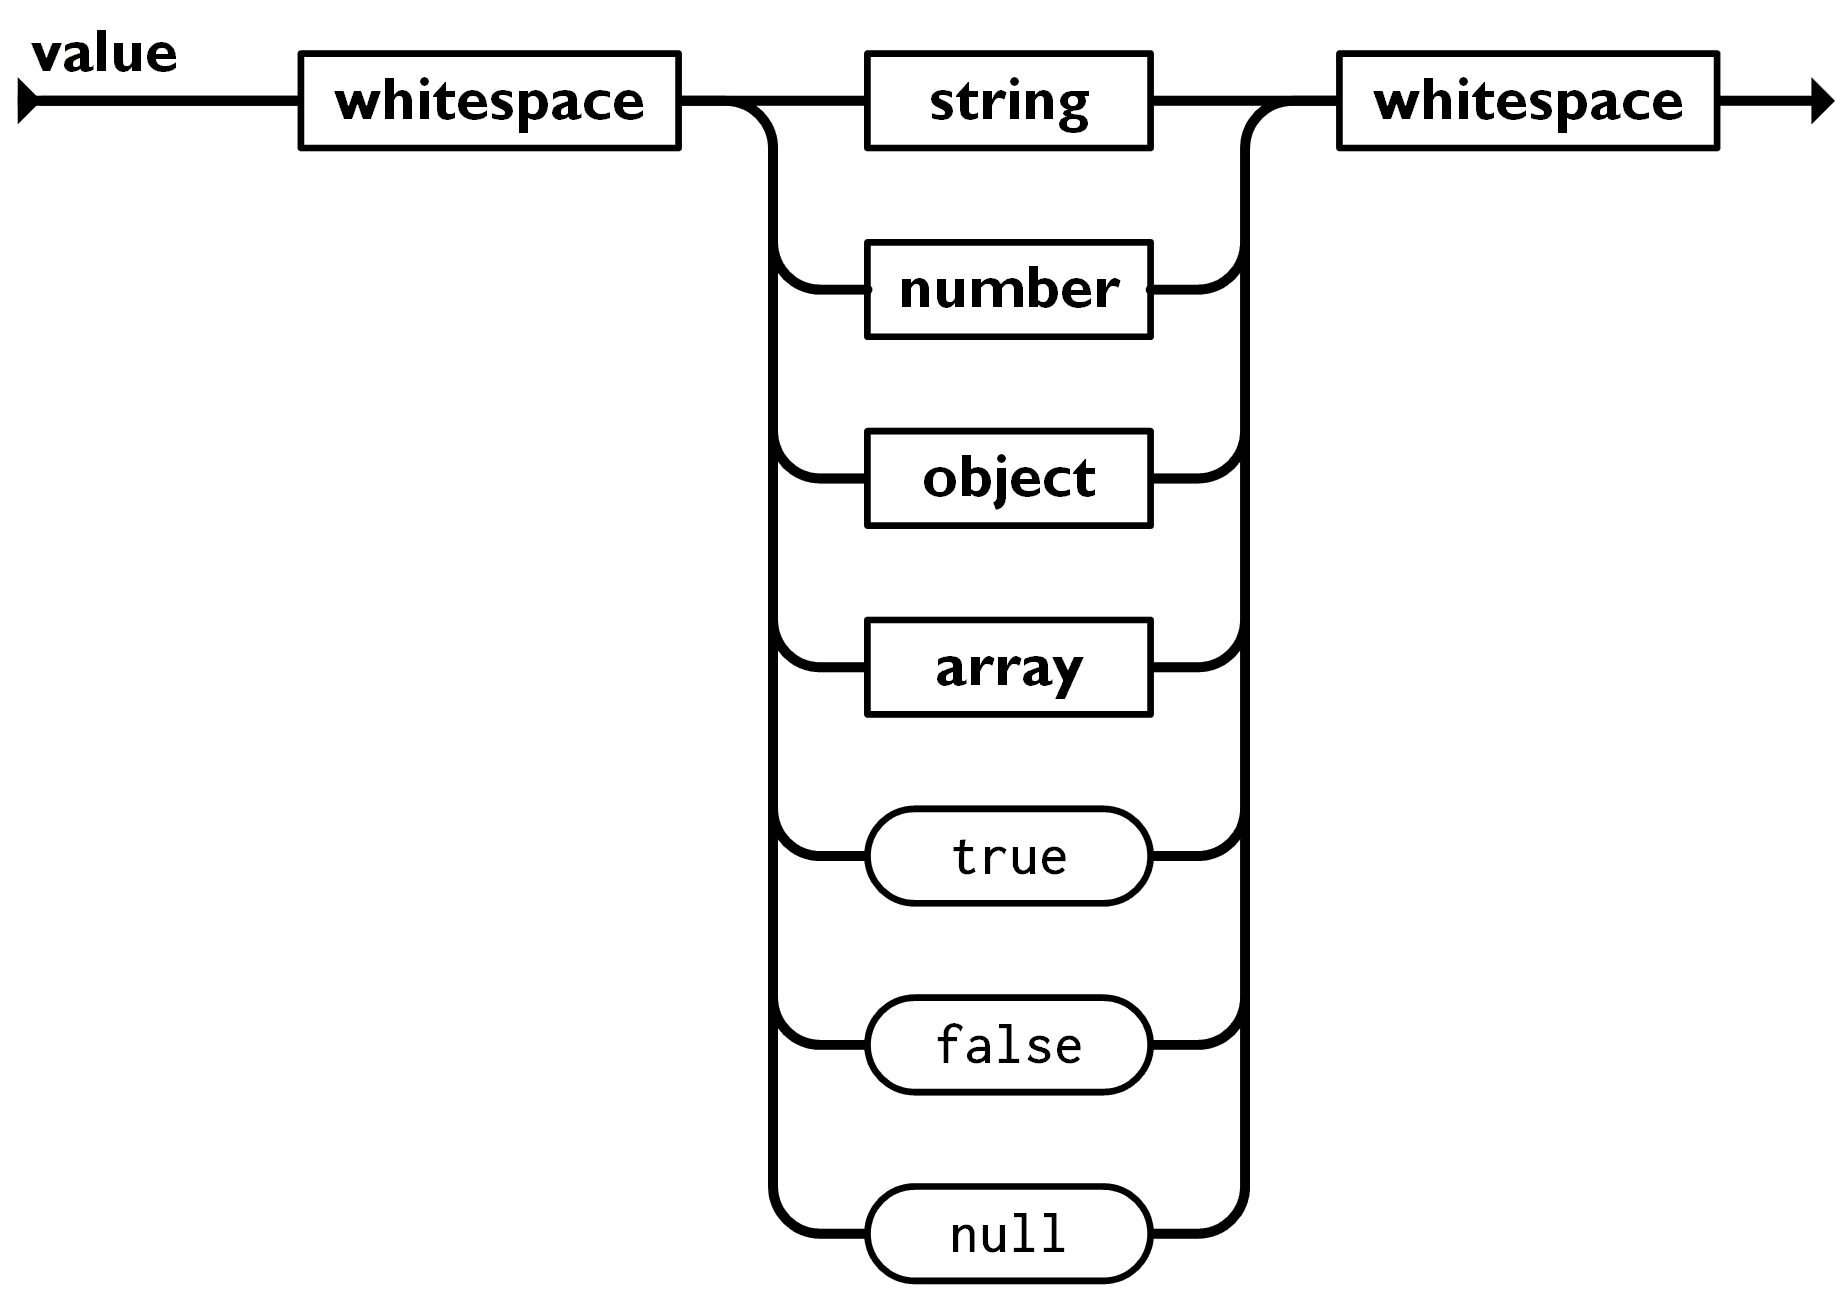
\includegraphics[scale=0.6]{value.png}
	      \newpage
	\item Строка \\
	      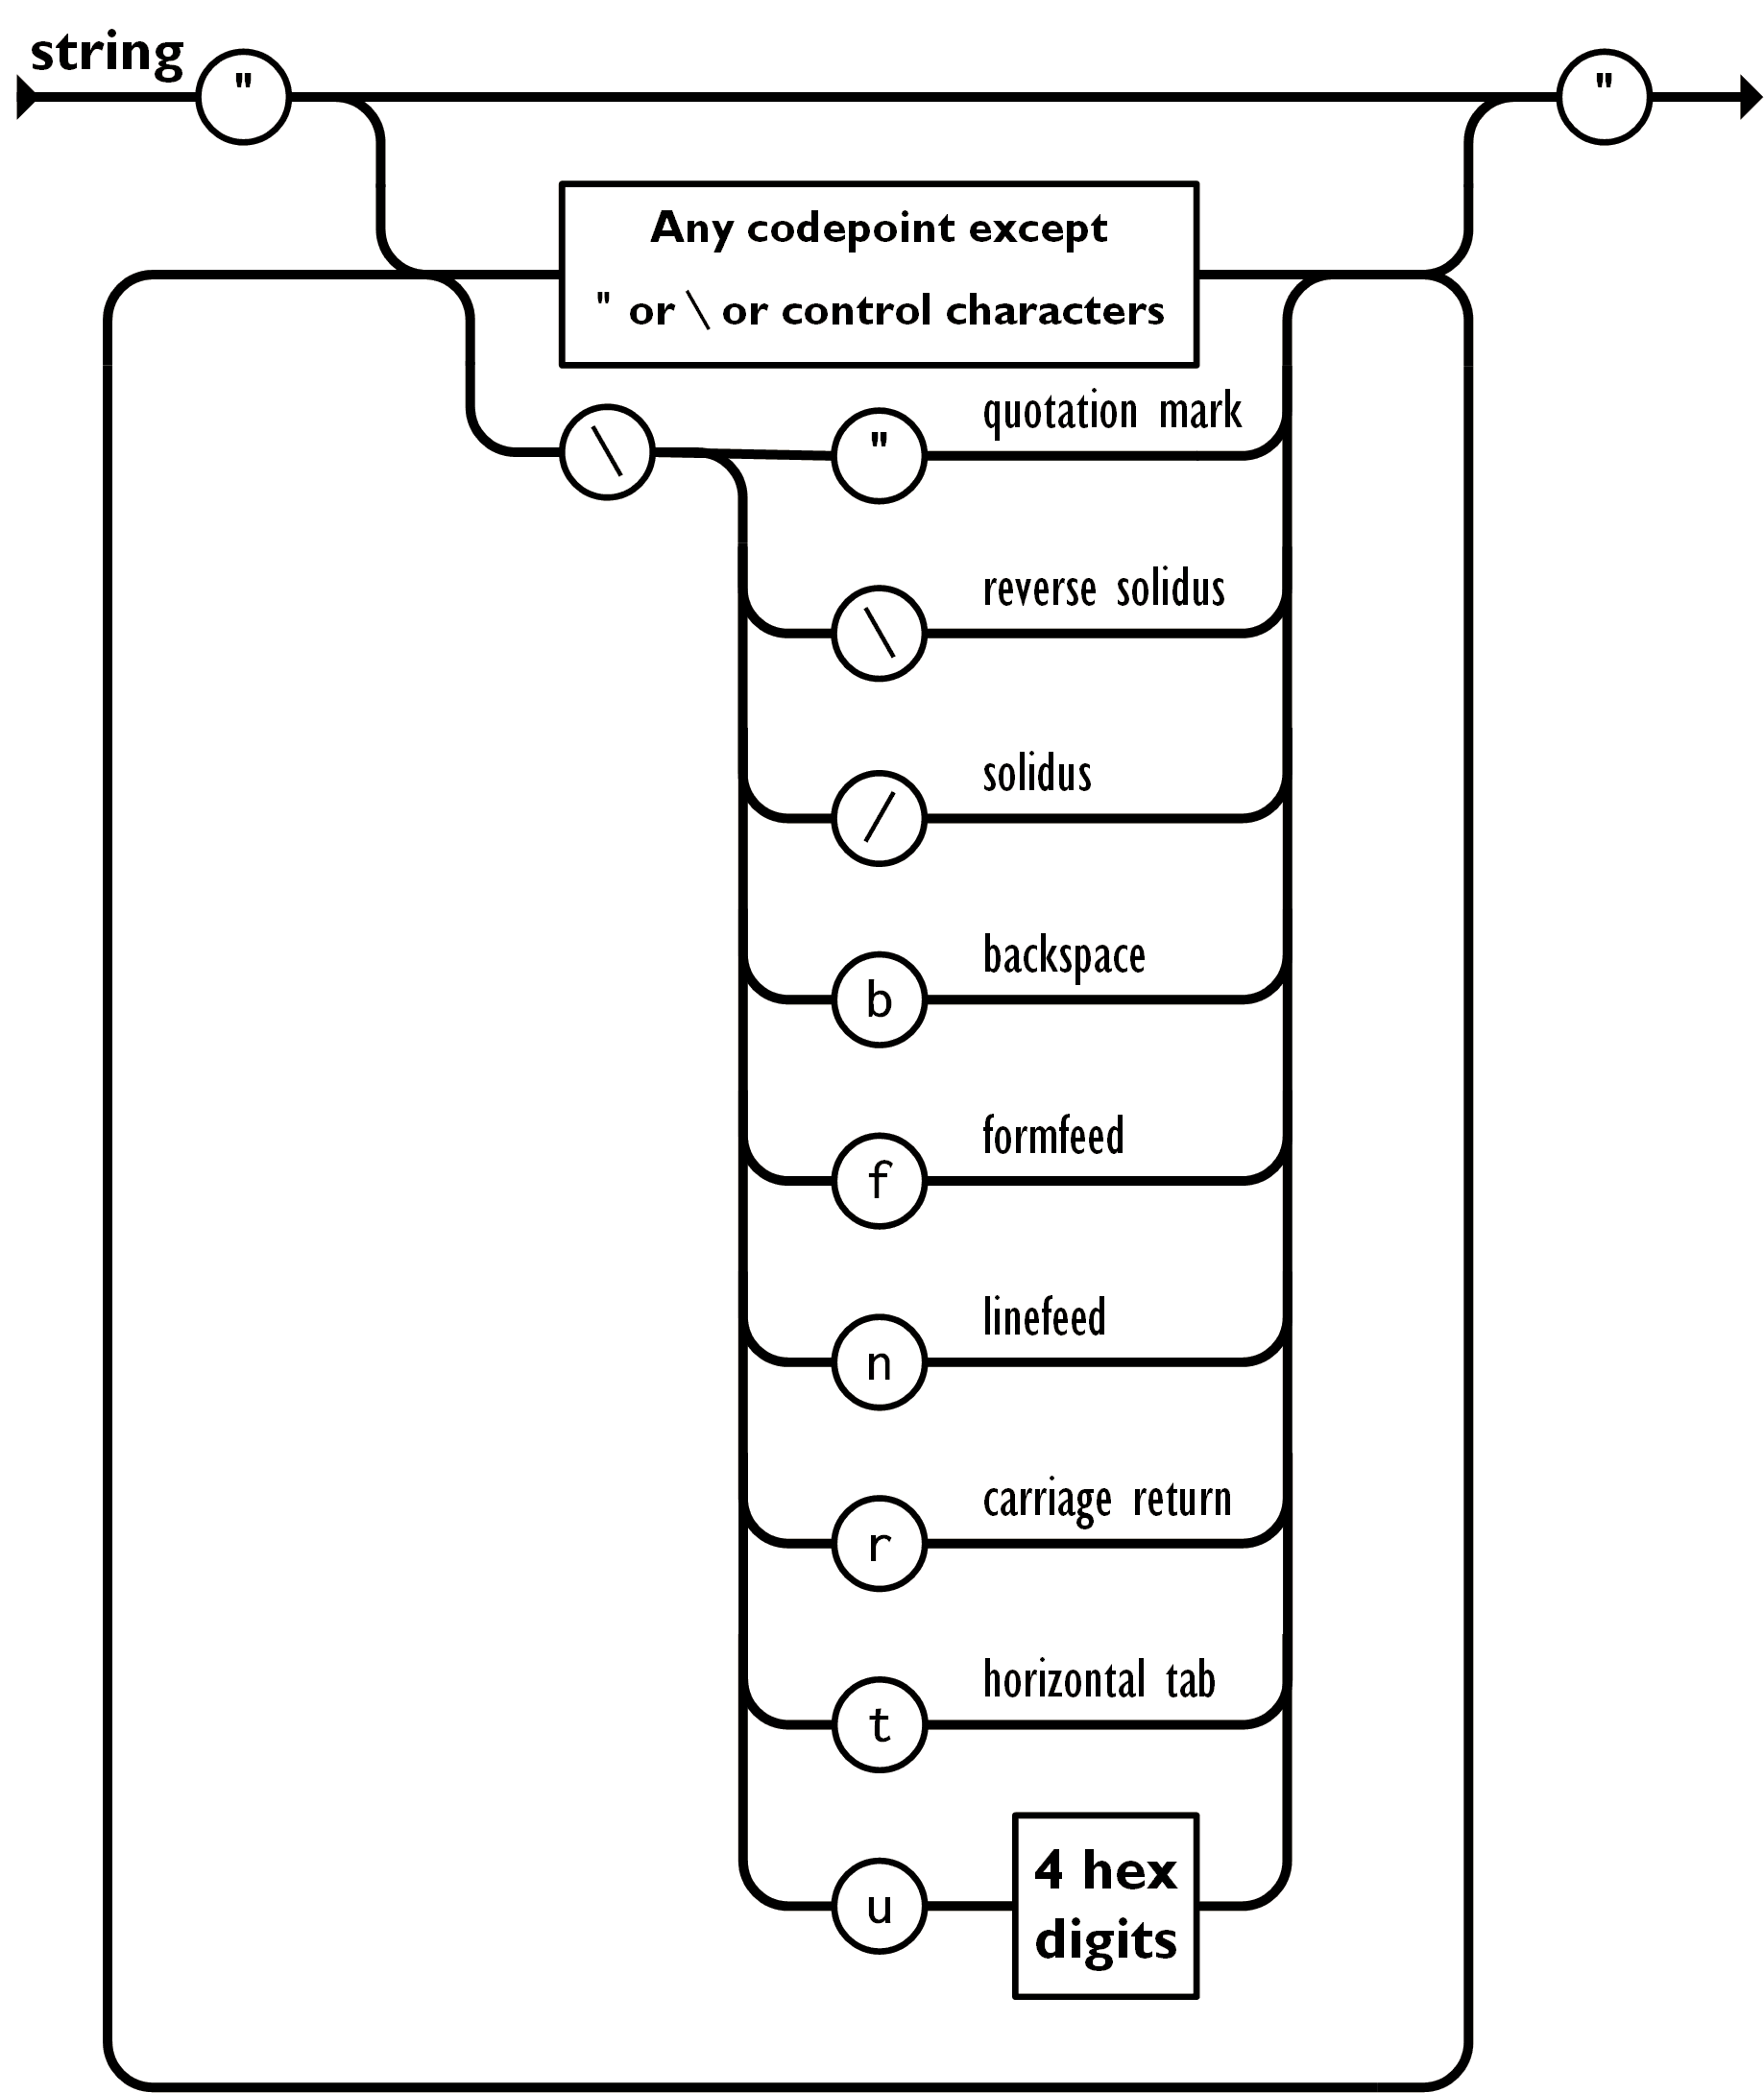
\includegraphics[scale=0.6]{string.png}
	      \newpage
	\item Объект \\
	      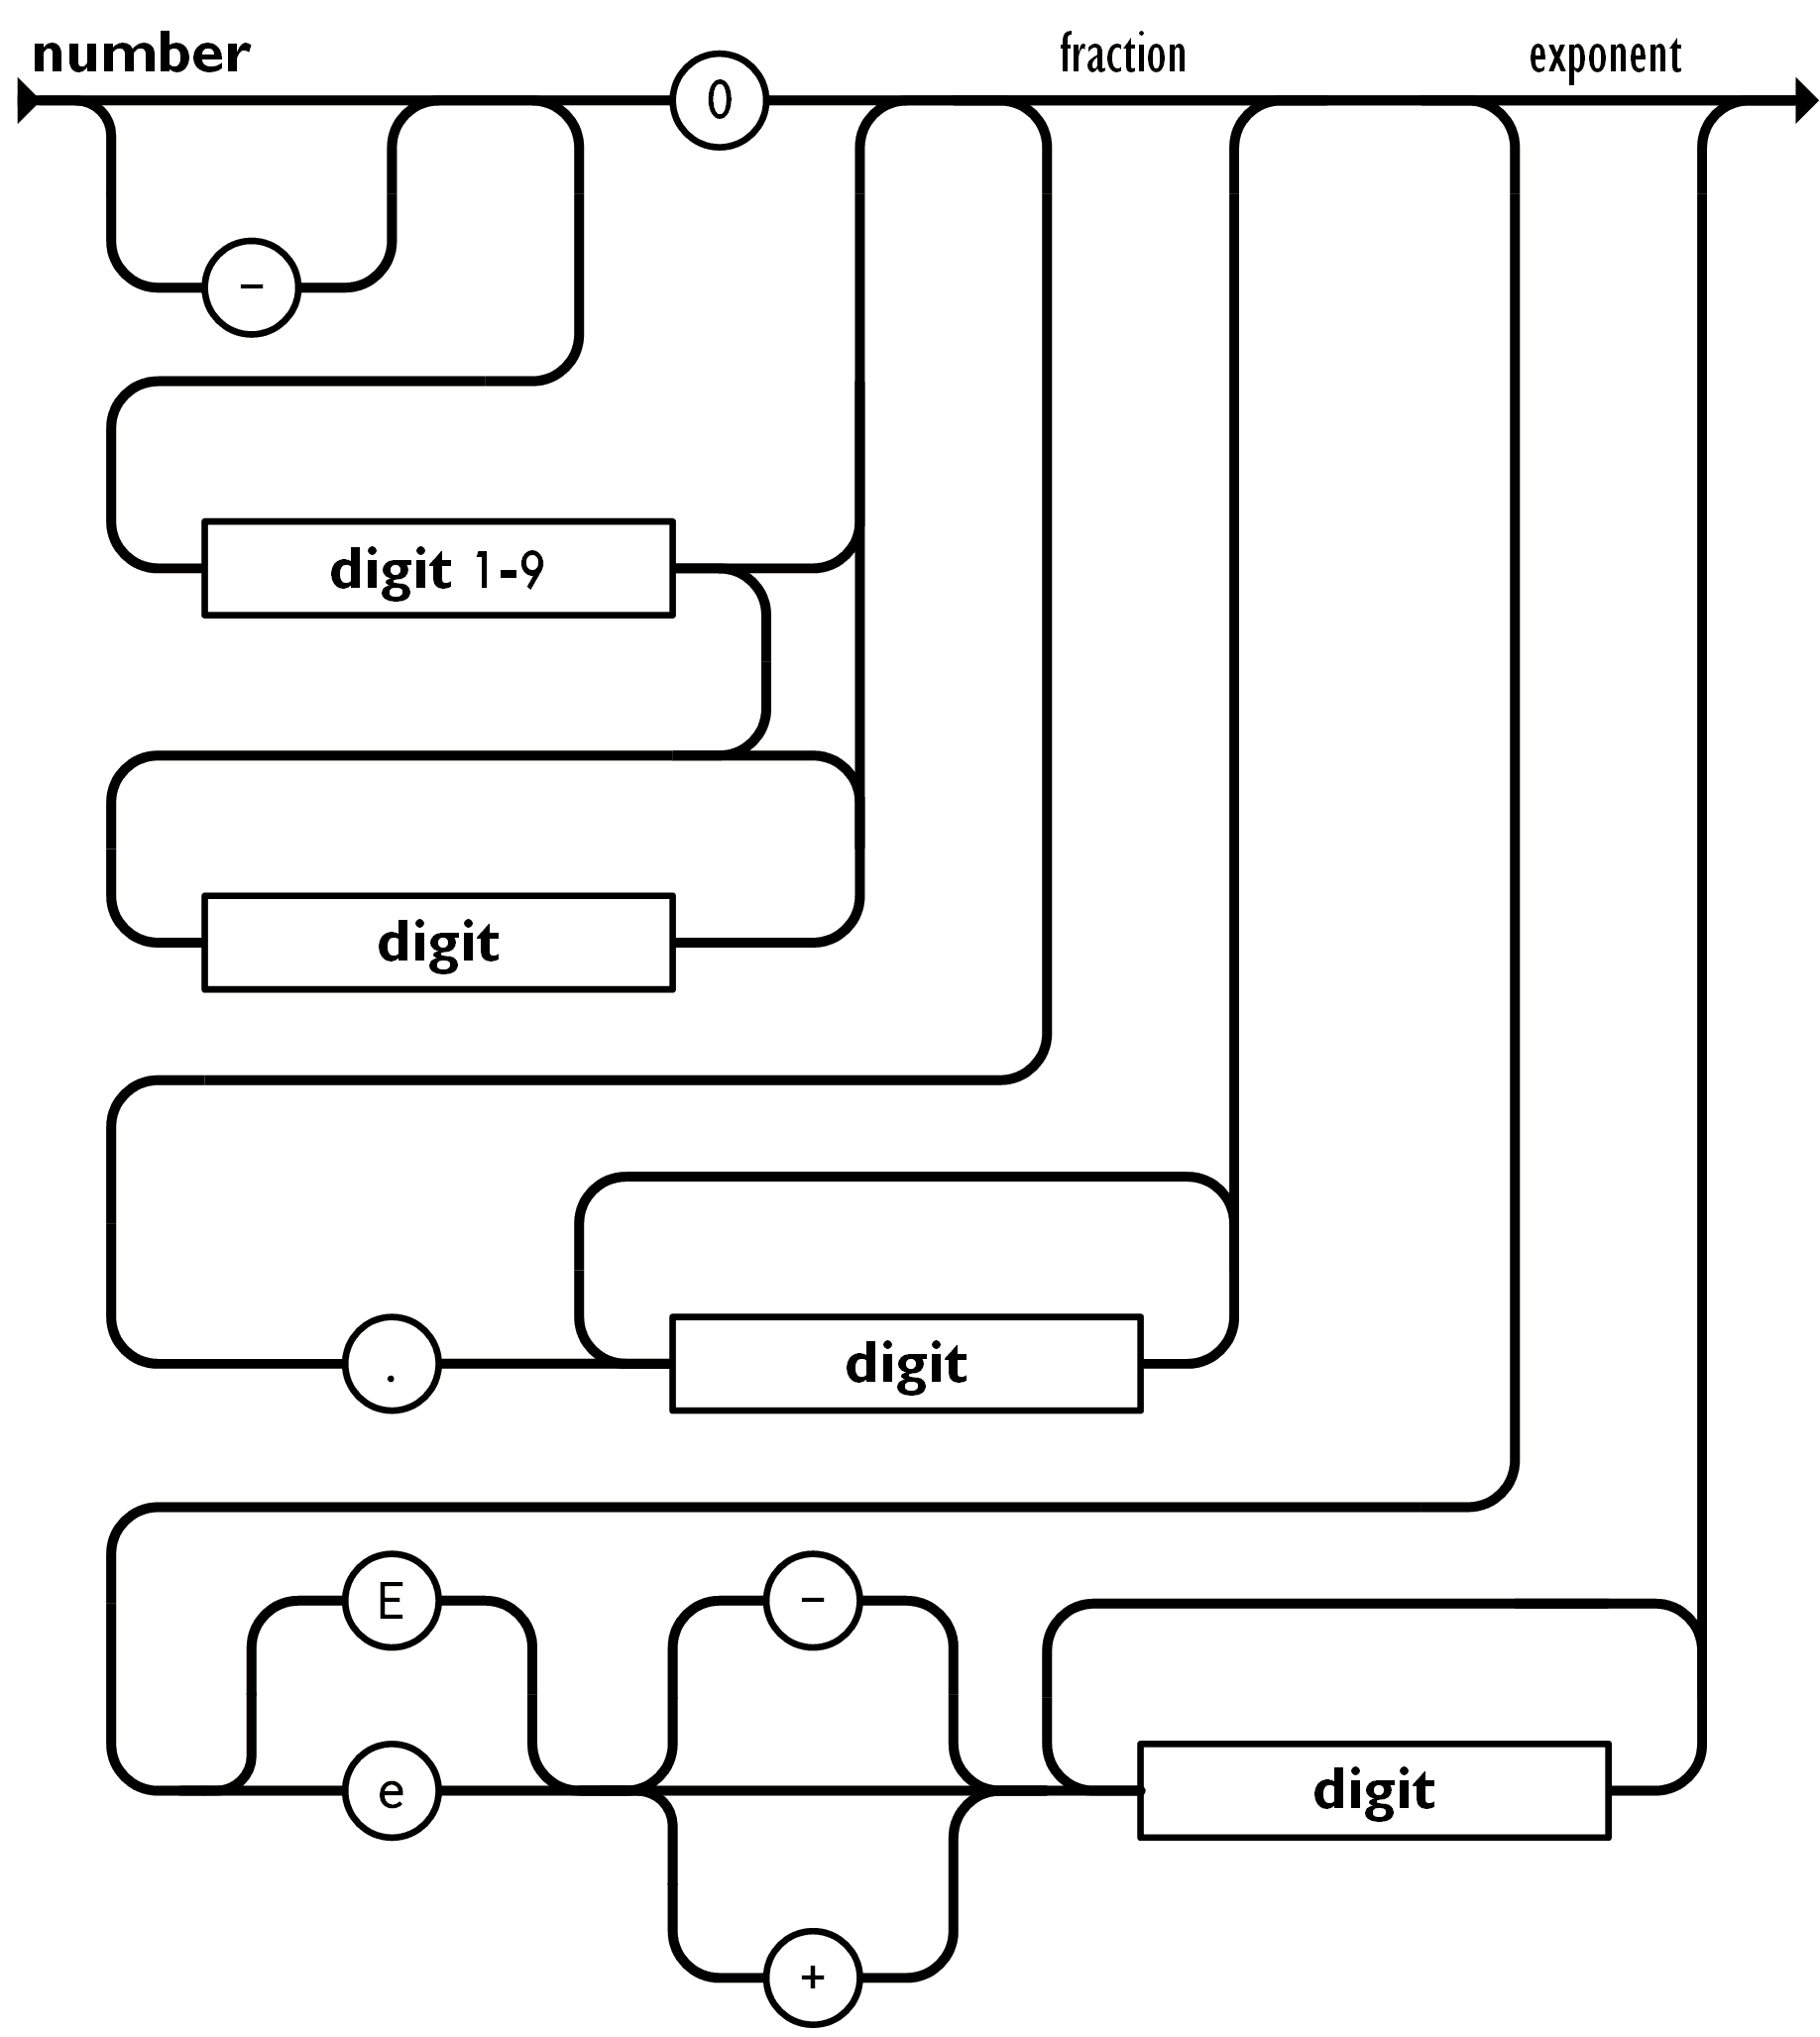
\includegraphics[scale=0.6]{number.png}
	\item Пробел \\
	      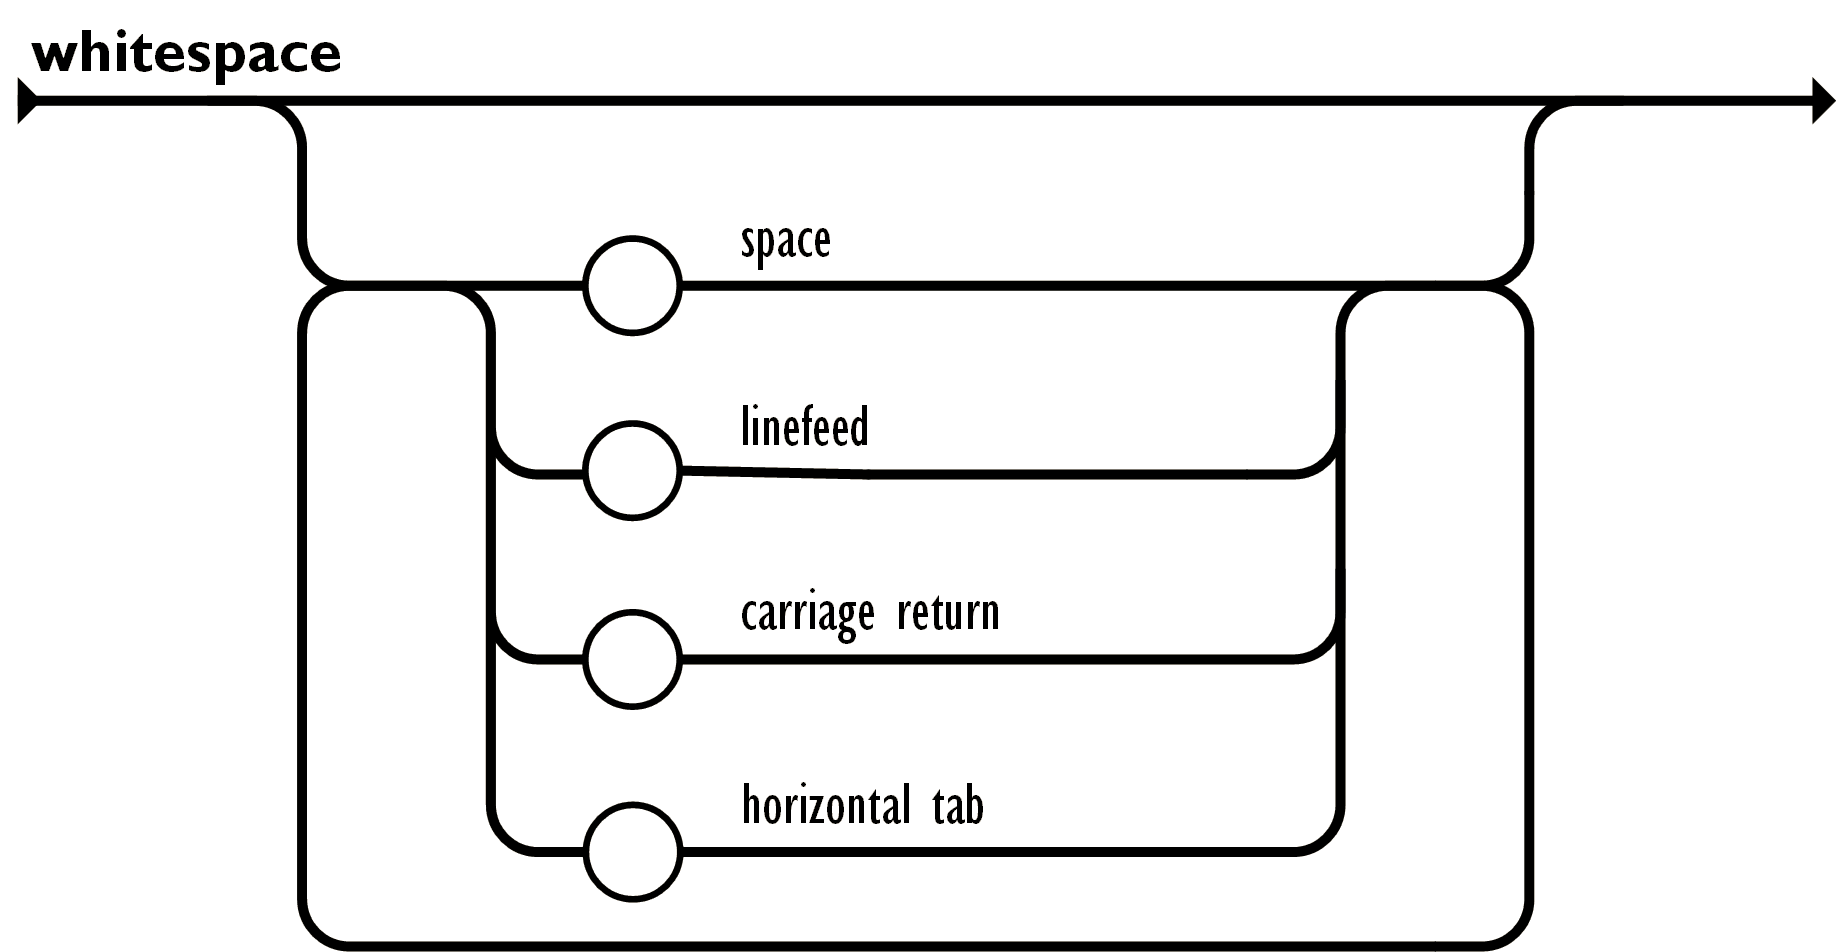
\includegraphics[scale=0.6]{whitespace.png}
\end{enumerate}

\newpage
\addcontentsline{toc}{section}{Список литературы}
\printbibliography
\end{document}
